\documentclass{beamer}
\usepackage{ctex}
\usepackage{graphicx}
\usepackage{multicol}
\usepackage{amsmath}
\usepackage{amsthm}
\usepackage{todonotes}
\usepackage{amssymb}
\usepackage{listings}

\usetheme{CambridgeUS}%这是主题
%\usecolortheme{whale}
\usecolortheme{dolphin}
\mode<presentation>
\title[Mantle Convection]{hw0}
\author{李昊臻,夏君毅,解士杰 }

\graphicspath{{pic/}}
%---------------------------标题页------------------------------
\begin{document}
\begin{frame}
我们的思路:怎么简单怎么来。\par
直接做向后差分离散,光滑化。作为一个多元函数梯度下降。\par
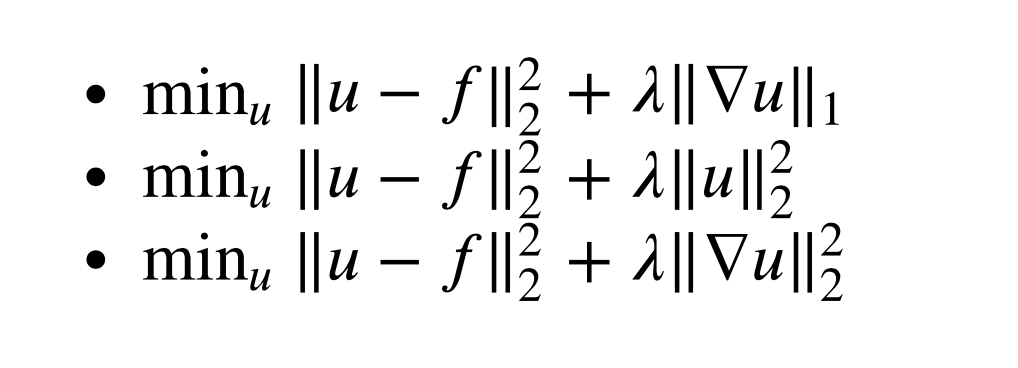
\includegraphics[width=8cm]{0.png}\\
第一个问题做光滑化化\\$\Vert \nabla u\Vert  = \Vert \sqrt{\vert\nabla u\vert^2 + \epsilon}\Vert $\\
第二个问题是各点解耦的,所以直接写答案就可以。\\
第三个本身就是光滑的。
\end{frame}


%---------------------------目录页------------------------------




\end{document}
